%\documentclass[printmode,oneside,eng]{mgr}  % do publikacji elektronicznej
\documentclass[printmode,eng]{mgr}  % do wydruku dwustronnego
%\documentclass[printmode,eng,draft]{mgr}  % do wydruku dwustronnego w~wersji roboczej

%----------------------| Input encoding configuration |

\usepackage[utf8]{inputenc}

%-------------------------| Typeface configuration |------------------------

%% Najpierw (chyba) należy wybrać czcionkę tekstu, potem matematyki

%% wybór czcionki Computer Concrete specjalnie zaprojektowanej do użycia 
%% z~czcionką matematyczną euler (nie ma ona niestety wersji bold - proponuje się więc użycie bolda z kroju
%%   Computer Modern Sans Serif)
%\usepackage{beton}             % ZALECANA DO SKŁADU TEKSTÓW PO ANGIELSKU
%\renewcommand{\bfdefault}{sbc} % to use Computer Modern Sans Serif demibold condensed fonts as bold 
%% choć może komuś bardziej podobać się będzie ten krój normalnej szerokości 
%\renewcommand{\bfdefault}{sb} % to use Computer Modern Sans Serif demibold fonts as bold 

%% alternatywny wybór Antykwy Półtawskiego - czcionki zaprojektowanej
%% specjalnie dla języka polskiego uwzględniającej jego rytm 
%\usepackage{antpolt}
%% alternatywny wybór Antykwy Toruńskiej - bardziej "współczesnej",
%% całkowicie polskiej czcionki
\usepackage{anttor}             % ZALECANA DO SKŁADU TEKSTÓW PO POLSKU
%\usepackage[math]{anttor}      % math włącza antykwę także w~matematyce
                                % ale chyba coś psuje :( (np. brak strzałek)

%% alternatywnie wybór czcionki URW Palladio
%\usepackage{newpxtext}  % Palatino font
%\linespread{1.05}  % Palatino needs more leading space (between lines)

%% ustawienie czcionki eulerowskiej do składu wyrażeń matematycznych
%\usepackage[euler-digits,small]{eulervm}
\usepackage{eulervm}

%% ustawienie czcionki bezszeryfowej Monospace (typewriter, code) font (last) - skład poleceń, wydruków programów
\usepackage[varqu,varl]{inconsolata}

%-------------------------| Sprawy polskie |------------------------

\usepackage[T1]{fontenc} % bez tego są złe znaki / { } w czcionce tt
                         % ale musi być użyty pakiet polski bez opcji
                         % wybierającej układ - gdy zamarkowane
                         % używamy pakiet polski z~opcją wyboru układu
\usepackage{polski}
%\usepackage[OT4]{polski} % domyślnie?

%---------------------------| Packetology |-------------------------

\usepackage{geometry}           % manipulowanie geometrią łamu
\usepackage{indentfirst}        % wcięcia akapitowe w pierwszych paragrafach rozdziałów
\usepackage[dvipsnames]{xcolor} % by mieć nazwy kolorów w~rodzaju \green
\usepackage{gensymb}
%% zmiana formatowania tytulariów
%\usepackage[raggedleft]{titlesec}

\usepackage[titles]{tocloft}    % do formatowani spisów

%% w razie potrzeby zmieniamy nieco odstępy przed rozdziałami i podrozdziałami w spisie
%% treści by uniknąć pojedynczego samotnego tytułu rozdziału/podrozdziału na dole/górze strony
%% i by ładnie się zmieściła notka o latechu
\addtolength{\cftbeforechapskip}{-0.9ex}
\addtolength{\cftbeforesecskip}{0.02ex}

%%modyfikacja odstępów między pozycjami w~bibliografii
\let\oldbibliography\thebibliography
\renewcommand{\thebibliography}[1]{%
  \oldbibliography{#1}%
  \setlength{\itemsep}{0pt plus 0.3ex}%
}

%% ustawienie maksymalnej liczby i obszaru dla obiektów pływających (rysunków, tabel)
\setcounter{topnumber}{3}
\setcounter{totalnumber}{4}
\renewcommand{\topfraction}{.8}

\usepackage{graphicx}                % dołaczanie i manipulowanie grafikami
\usepackage[export]{adjustbox}       % więcej komend operujących na "pudełkach"
\usepackage[caption = false]{subfig} % obsługa rysunków z częściami

\usepackage{svg}                % dołączanie grafik w formacie svg
%\usepackage[inkscapepath=svgdir]{svg}  % w nowszych wersjach

\usepackage{tikz}               % dołączanie grafik w formacie TikZ
\usepackage{makecell}           % trochę tikzowej magii
    \tikzstyle{block} = [draw, fill=blue!20, rectangle, 
     minimum height=3em, minimum width=6em]
    \tikzstyle{sum} = [draw, fill=blue!20, circle, node distance=3.5cm]
    \tikzstyle{input} = [coordinate]
    \tikzstyle{output} = [coordinate]
    \tikzstyle{pinstyle} = [pin edge={to-,thin,black}]    
    \usetikzlibrary{arrows,automata,calc,positioning}
\usepackage{standalone}  

\usepackage{pgfplots}           % do robienia wykresów 
\pgfplotsset{compat=1.5}        %% why 1.5? pl. update

\usepackage{mathtools}          % doskonałe pakiety rozszerzające do matematyki
\usepackage{amssymb, amsfonts}  % mathtools zastępuje amsmath (naprawione błedy, dodane rozszerzenia) 
\usepackage{wasysym}            % trochę więcej różnych symboli (buźki)
%\usepackage[fleqn]{mathtools}  % równania w wersji dosuniętej w lewo
%% automatyczne numerowanie jedynie tych równań, do których są odwołania w~tekście
%\mathtoolsset{showonlyrefs=true}

%% symbole do oznaczania stopek w~miejsce liczb
\renewcommand{\thefootnote}{\fnsymbol{footnote}}
%% powtórzone z latex.ltx - w przeciwnym razie znika symbol \textbardbl przy
%% wybranej Antykwie Toruńskiej (sprawdzić co z innymi definicjami z omsenc.def,
%% sprawdzić czy też przy innych czcionkach)
\DeclareTextSymbolDefault{\textbardbl}{OMS}
%% automatyczne resetowanie wartości licznika stopek użyteczne przy użyciu symboli
%% do oznaczania stopek w~miejsce liczb (liczba dostępnych symboli wynosi tylko 9)
\usepackage{etoolbox,pdftexcmds}
\makeatletter
\patchcmd{\footnote}
  {\stepcounter\@mpfn}
%  {\stepcounter\@mpfn\check@overflow\@mpfn} %%było w~przykładzie
  {\stepcounter\@mpfn\check@overflow}
  {}{}
\newcommand{\check@overflow}{%
  \ifnum\pdf@strcmp{\@mpfn}{footnote}=\z@
    \ifnum\value{footnote}>8  %tu było 9, ale czasami nie resetowało poprawnie
      \setcounter{footnote}{1}%
    \fi
  \fi
}
\makeatother

\usepackage{hyperref}           % obsługa aktywnych odnośników i hypertekstu
\usepackage{url}                % obsługa adresów url

%% pakiet minted do wydruków programów
%% 'minted' gives much better highlight then the default listings,
%% but it reqires Python with Pygments (check the documentation of minted)
%% it also requires passing '-shell-escape' option to pdflatex during compilation
\usepackage[%
  cache=false,
  chapter,
  %    outputdir=build,  % if building in separate directory, this must be included
                         % ale nie zawsze działa poprawnie :( 
    newfloat  % required if multi-page floating listings are needed (see below)
]{minted}  % (note: from my experience must be loaded before 'csquotes')
%% by wybrać inny styl - lista dostępnych styli: pygmentize -L styles
%\usemintedstyle{igor}
\SetupFloatingEnvironment{listing}{name=Wydruk}
%% kolor tła używany w~wydrukach
\definecolor{OurListingBackground}{rgb}{0.95,0.95,0.95}
%% fix the minted@colorbg environment bug
\makeatletter
\renewenvironment{minted@colorbg}[1]
 {\def\minted@bgcol{#1}%
  \noindent
  \begin{lrbox}{\minted@bgbox}
  \begin{minipage}{\linewidth-2\fboxsep}}
 {\end{minipage}%
  \end{lrbox}%
  \setlength{\topsep}{\bigskipamount}% set the vertical space
  \trivlist\item\relax % ensure going to a new line
  \colorbox{\minted@bgcol}{\usebox{\minted@bgbox}}%
  \endtrivlist % close the trivlist
 }
\makeatother

%%pakiet do robienia notatek w trakcie pracy
\usepackage{todonotes}
\makeatletter   %spolszczenie
\renewcommand{\@todonotes@todolistname}{Do zrobienia}
\renewcommand{\@todonotes@MissingFigureText}{Rysunek}
\renewcommand{\@todonotes@MissingFigureUp}{Brakujący}
\renewcommand{\@todonotes@MissingFigureDown}{rysunek}
\makeatother

%% dodaje w pliku wynikowym klucze etykiet i referencji - wygodne przy pracy nad tekstem
%\usepackage{showkeys}

%%inne przydatne
%\usepackage{fancyhdr}
%\usepackage{fancyvrb}
%\usepackage{lipsum}  
%\usepackage{listings}

%-----------------------| End of packetology |----------------------

%---------------------------| Tytularia |---------------------------

% Zmień dane stosownie do tytułu i autora pracy tutaj
% ALE TEŻ I W POLECENIU \pdftitle NIECO PONIŻEJ! (Hyper data general configuration)
\author{Maciej Gaik}
\title{Projekt budowy odwróconego wahadła matematycznego}
\engtitle{Design and construction reversed pendulum}
\supervisor{Dr inż. Mateusz Cholewiński,\\ Katedra Cybernetyki i~Robotyki}
\field{Automatyka i~Robotyka (AIR)}
\specialisation{Robotyka (ARR)}
\date{2020}

%-------------------------| Hyper data general configuration |------------------------

\hypersetup{unicode,
   pdfpagemode=UseOutlines,   % otwiera dokument w trybie jednej strony
   pdfpagelayout=SinglePage,  %
   pdfstartpage=1,            % na podanej stronie
   bookmarksopen=true,        % rozwinięcie zakładek
   bookmarksopenlevel=1,      % do jakiego poziomu
   colorlinks=true,      % kolorowanie odnośników zamiast ramki wokół nich
   citecolor=cyan,       % kolor odnośników do bibliografii, domyślnie zielony
   filecolor=red,        % kolor odnośników do lokalnych plików, domyśnie magenta
   linkcolor=blue,       % kolor odnośników wewnętrznych, domyślnie czerwony
   menucolor=green,      % kolor pozycji menu Acrobata, domyślnie czerwony
   urlcolor=blue,        % kolor odnośników do adresów internetowych, domyślnie cyan
                              % DANE DOKUMENTACJI
   pdftitle={Bąk jaki jest każdy widzi. Studium zachowań - Przykład
    i~wytyczne formatowania pracy dyplomowej},
   pdfauthor={Roberto Orozco, Robert Muszyński},
   pdfsubject={Praca dyplomowa inżynierska - przykład i~wytyczne},
   pdfkeywords={bąk, Lagrange top, Euler top, praca dyplomowa, formatowanie, wytyczne}
}

%-------------------------| Geometria strony |-----------------------------

\geometry{
    top = 25mm,
    headheight = 15mm,
    headsep = 3mm,
    textheight = 24cm,
    textwidth = 16cm,
}

%---------------------| Frequently used commands definitions |-------------------

\newcommand{\red}{\color{red}}
\def\BibTeX{{\rm B\kern-.05em{\sc i\kern-.025em b}\kern-.08em
    T\kern-.1667em\lower.7ex\hbox{E}\kern-.125emX}}

\newtheorem{uwaga}{Uwaga}
\newtheorem{twr}{Twierdzenie}
%------------------------------------| END |-------------------------------------

%----------------------------| Math symbols definition |-------------------------

\newcommand{\angmom}{\boldsymbol{m}}
\newcommand{\bdvelo}{\boldsymbol{\omega}_B}
\newcommand{\grav}{\boldsymbol{g}}
\newcommand{\lagran}{L(\boldsymbol{q},\boldsymbol{\dot{q}})}
\newcommand{\COMvec}{\boldsymbol{r}_B}
\newcommand{\ee}{\boldsymbol{e}}
\newcommand{\FF}{\boldsymbol{F}}
\newcommand{\xx}{\boldsymbol{x}}
\newcommand{\qq}{\boldsymbol{q}}
\newcommand{\RR}{\boldsymbol{R}}
\newcommand{\TT}{\boldsymbol{T}}
\newcommand{\pp}{\boldsymbol{p}}
\newcommand{\iner}{\boldsymbol{I}_B}
\newcommand{\vv}{\boldsymbol{v}}
\newcommand{\bbs}{\boldsymbol}
\DeclareMathOperator{\const}{const}
\DeclareMathOperator*{\rank}{rank} 

\graphicspath{{figures/chapter_01/}{figures/chapter_02/}{figures/chapter_03/}{figures/chapter_04/}}


\begin{document}

\pdfbookmark{Strona tytułowa}{tytul}
\maketitle
%% informacja o sposobie udostępniania tego dokumentu
\thispagestyle{empty}
\mbox{}
\vfill

\noindent
{\bf Robert Muszyński, Roberto Orozco}\\
{\bf Wrocław 2019}\\[2ex]
  
\includegraphics[width=0.18\textwidth]{figures/CC-BY-SA_icon_svg.png}\hfill
\begin{minipage}[b]{0.79\textwidth}
 \small Szablon jest dostępny na licencji Creative Commons: \emph{Uznanie au\-tor\-stwa-Na tych samych warunkach 4.0 Polska}
\end{minipage}\vspace{2ex}

\noindent
{\normalsize Utwór udostępniany na licencji Creative Commons: uznanie
  autorstwa, na tych samych warunkach. Udziela się zezwolenia do
  kopiowania, rozpowszechniania i/lub modyfikacji treści utworu
  zgodnie z zasadami w/w licencji opublikowanej przez Creative
  Commons. Licencja wymaga podania oryginalnego autora utworu, a
  dystrybucja materiałów pochodnych może odbywać się tylko na tych
  samych warunkach (nie można zastrzec, w jakikolwiek sposób
  ograniczyć, ani rozszerzyć praw do nich). Tekst licencji jest
  dostępny pod adresem:
  \url{https://creativecommons.org/licenses/by-sa/4.0/legalcode.pl}.}


\cleardoublepage
\pdfbookmark{\contentsname}{Contents}
\tableofcontents            %spis treści
\markboth{\contentsname}{\contentsname}
%%\newpage
%\thispagestyle{empty}
%\cleardoublepage
%\thispagestyle{plain}

\mbox{}\vfill\hfill
\begin{minipage}{0.5\linewidth} 
  {\tiny \noindent Do składu pracy wykorzystano system przygotowania
    dokumentów~\LaTeX, opracowany przez
    L.~Lamporta\index{latex>\LaTeX} [Lam94], będący nakładką
    systemu \TeX, [Knu86a,Knu86b].  Matematyczne czcionki o nazwie
    {AMS Euler}, których używamy w tej pracy, zostały przygotowane
    przez H.\ Zapfa [KZ86], przy współpracy z~D.\ Knuthem i~jego
    studentami, na zlecenie Amerykańskiego Towarzystwa Matematycznego.
    %% Przy wybranej Antykwie Toruńskiej/Półtawskiego odznacz odpowiednio poniższe
    Wybrane czcionki składu tekstu, Antykwa Toruńska [Now97] -- jeden
    %Wybrane czcionki składu tekstu, Antykwa Półtawskiego [Now99] -- jeden
    z~nielicznych krojów pisma zaprojektowany specjalnie dla języka
    polskiego w~sposób uwzględniający jego rytm -- w~odczuciu autora
    doskonale współgrają z~kształtem czcionki {AMS Euler}, pozwalając
    na uzyskanie harmonijnej całości.
    % %% Przy wybranych czcionkach Concrete odznacz poniższe
    % Czcionki składu tekstu, zwane {Concrete Roman} i {Concrete
    %   Italic}, należące do knuthowskiej rodziny czcionek {Computer
    %   Modern}, zostały specjalnie przystosowane do kształtu czcionki
    % {AMS Euler} na potrzeby książki [GKP96].
    % %% Przy wybranych czcionkach URW Palladio odznacz poniższe
    % Czcionka składu tekstu, zwana URW Palladio jest klonem zapfoskiej rodziny
    % czcionek o~nazwie Palatino [LPn05] i~zdaniem autora świetnie współgra
    % z~kształtem czcionki {AMS Euler}.
    Składu bezszeryfowego tekstu maszynowego dokonano z~użyciem
    opracowanej przez R. Leviena czcionki o~nazwie Inconsolata
    [Lev15]\footnote{\red\tiny Chyba warto takie informacje szerzyć}.


\vspace{-4mm}

 \makeatletter
\renewenvironment{thebibliography}[1]
     {%
        \tiny%
      \list{\@biblabel{\@arabic\c@enumiv}}%
           {\settowidth\labelwidth{\@biblabel{#1}}%
\setlength{\itemsep}{2.5mm}
            \leftmargin\labelwidth
            \advance\leftmargin\labelsep
            \@openbib@code
            \usecounter{enumiv}%
            \let\p@enumiv\@empty
            \renewcommand\theenumiv{\@arabic\c@enumiv}}%
      \sloppy\clubpenalty4000\widowpenalty4000%
      \sfcode`\.\@m\vspace{5mm}}
     {\def\@noitemerr
       {\@latex@warning{Empty `thebibliography' environment}}%
      \endlist}

\makeatother

\begin{thebibliography}{Knu86b}

% %% Odmarkować pozycję gdy wybrane czcionki Concrete
% \bibitem[GKP96]{GKP96loc}
% R.~L. Graham, D.~E. Knuth i O.~Patashnik,
% \newblock { Matematyka konkretna}.
% \newblock PWN, Warszawa, 1996.\vspace{-3mm}

\bibitem[Knu86a]{Knuth86loc}
D.~E. Knuth,
\newblock { The \TeX book, volume {A} of Computers and Typesetting}.
\newblock Addison-Wesley, Reading, 1986.\vspace{-3mm}

\bibitem[Knu86b]{Knuth86aloc}
D.~E. Knuth,
\newblock { \TeX: {The} Program, volume {B} of Computers and Typesetting}.
\newblock Addison-Wesley, Reading, 1986.\vspace{-3mm}

\bibitem[KZ86]{KnZa89loc}
D.~E. Knuth i H.~Zapf,
\newblock {AMS} {Euler} --- {A} new typeface for mathematics.
\newblock { Scholary Publishing}, {20}:131--157, 1986.\vspace{-3mm}

\bibitem[Lam94]{Lamport94loc}
L.~Lamport,
\newblock { \LaTeX: A Document Preparation System}.
\newblock Addison-\mbox{-Wesley}, Reading, 1994.\vspace{-3mm}

\bibitem[Lev15]{Levien15loc}
R.~Levien,
\newblock {Inconsolata}.
\newblock \url{https://levien.com/type/myfonts/inconsolata.html}, 2015.\vspace{-3mm}

% %% Odmarkować pozycję przy wybranej czcionce URW Palladio
% \bibitem[LPn05]{LinotypePalatino05loc}
% Linotype Palatino nova: A classical typeface redesigned by Hermann Zapf,
% \newblock Linotype Library GmbH, 2005.\vspace{-2mm}

%% Odmarkować pozycję przy wybranej Antykwie Toruńskiej
\bibitem[Now97]{nowacki97loc}
J.~Nowacki,
\newblock {Antykwa} {Toruńska} -– od początku do końca polska czcionka.
\newblock {\em Biuletyn Polskiej Grupy Użytkowników Systemu \TeX}, 9:26--27,
  \nolinebreak1997.\vspace{-2mm}

% %% Odmarkować pozycję przy wybranej Antykwie Półtawskiego
% \bibitem[Now99]{nowacki99}
% J.~Nowacki,
% \newblock Piórkiem i {MetaPost-em}, czyli {Antykwa} {Półtawskiego}.
% \newblock {\em Biuletyn Polskiej Grupy Użytkowników Systemu \TeX}, 12:49--53,
%   \nolinebreak1999.\vspace{-2mm}

\end{thebibliography}
}
\end{minipage}
       %notka o systemie składu i czcionkach
%\input{sources/font-note}   %przykładowa wersja angielska notki

%% część właściwa dokumentu
\chapter{Wstęp}
\label{wstep}
\chapter{Preliminaria matematyczne}\label{ch:02}

\section{Wprowadzenie}\label{sec:intromat}

Odwrócone wahadło to przykład wahadła, które środek swojej masy ciężkości ma powyżej punktu obrotu, przez co jest układem wysoce niestabilnym. Układ taki charakteryzuje się dwoma punktami swobody: punkt obrotu pręta i poruszający się poziomo wózek, oraz tylko jednym wejściem sterującym, które odpowiada za ruch poziomy układu. Problem polega na takim sterowaniu wózkiem w osi poziomej, aby wahadło było utrzymane w osi pionowej, bądź oscylowało wokół punktu równowagi, bez opadania w dół. Sterowanie odbywa się poprzez przykładanie siły tylko do wózka, na wahadło działała tylko siła grawitacji i jej składowe, a jego punkt obrotu jest w pełni swobodny. 

\section{Model matematyczny} \label{sec:modelmat}

Układ odwróconego wahadła został przedstawiony na rysunku \ref{fig:draw}. Rzeczywisty układ wahadła uwzględnia moment bezwładności pręta, który w tym modelu został zastąpiony przez pręt o pomijalnie małej masie i niewielkiej masie \textit{m} na jego końcu. 

\begin{figure}
    \centering
    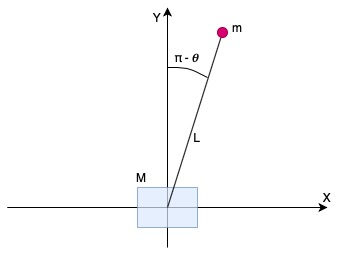
\includegraphics[scale=0.8]{praca_dyplomowa_wzor/figures/pendulum_draw.jpg}
    \caption{Układ odwróconego wahadła}
    \label{fig:draw}
\end{figure}

Współrzędne końca wahadła są opisane przez:
\begin{equation}
    \begin{cases}
    x_{p}=x+L\sin{\Theta}\\ 
    y_{p}=L\cos{\Theta}
    \end{cases}
\end{equation}
gdzie \textit{x} to współrzędna masy \textit{M}. Składowe prędkości masy \textit{m} można wyznaczyć przez pierwsze pochodne jego współrzędnych: 
\begin{equation}
    \begin{cases}
    \dot{x}_{p}=\dot{x}+L\dot{\Theta}\cos{\Theta}\\
    \dot{y}_{p}=-L\dot{\Theta}\sin{\Theta}
    \end{cases}
    \label{skladowe}
\end{equation}

Energia kinetyczna kinetyczna układu może być wyrażone przez równanie \ref{ekin}, przy założeniu, że ramię wahadła ma pomijalnie małą masę, a tym samym jego moment bezłwadności jest równy 0.
\begin{equation}
    K=\frac{1}{2}M{v_{1}}^{2}+\frac{1}{2}m{v_{2}}^{2},
    \label{ekin}
\end{equation}
gdzie \textit{v\textsubscript{1}} i \textit{v\textsubscript{2}} to odpowiednio prędkosci mas \textit{M} i \textit{m} i wynoszą:
\begin{equation}
    \begin{array}{l}
         v_1=\dot{x} \\
         v_2=\sqrt{\dot{x_p}^{2}+\dot{y_p}^{2}}
    \end{array}
\end{equation}
Korzystajac z wyprowadzenia \ref{skladowe} kwadrat prędkość \textit{v\textsubscript{2}} mozna wyraznić następujaco: 
\begin{equation}
    v_2^2=(\dot{x}+L\dot{\Theta}cos(\Theta))^{2}+(-L\dot{\Theta}sin(\Theta))^{2}=\dot{x}^2+2L\dot{\Theta}\dot{x}\cos{\Theta}+L^2\dot{\Theta}^2
\end{equation}
Zatem energia kinetyczna układu jest równa:
\begin{equation}
    K=\frac{1}{2}(M+m)\dot{x}^2+mL\dot{\Theta}\dot{x}\cos{\Theta}+\frac{1}{2}mL^2\dot{\Theta}^2
\end{equation}
,,Energia potencjalna układu pochodzi od siły grawitacji działającej na kulę" \cite{TchMu18} i wyraża się wzorem:
\begin{equation}
    V=mgL\cos{\Theta}
\end{equation}

Łącząc wyprowadzone równania na energię kinetyczną i potencjalną otrzymamy lagranżian:

\begin{equation}
    L=K-V=\frac{1}{2}(M+m)\dot{x}^2+mL\dot{\Theta}\dot{x}\cos{\Theta}+\frac{1}{2}mL^2\dot{\Theta}^2-mgL\cos{\Theta}
\end{equation}

Do wyznaczenia równań Eulera-Lagrange’a potrzebne są następujące pochodne:
\begin{equation}
        \begin{array}{l}
         \frac{\partial L}{\partial x}=0 \\ \\
         \frac{\partial L}{\partial \Theta}=mg\sin{\Theta} \\ \\
         \frac{\partial L}{\partial \dot{x}}=(M+m)\dot{x}+mL\dot{\Theta}\cos{\Theta} \\ \\
         \frac{\partial L}{\partial \dot{\Theta}}=mL\dot{x}\cos{\Theta}+mL^2\dot{\Theta}
    \end{array}
\end{equation}
\chapter{Budowa urządzenia}

\section{Konstrukcja}

Część mechaniczna urządzenia została zamodelowana w programie Solidworks, dzięki czemu ustalono jakie elementy konstrukcyjne są potrzebne oraz czy nie występują kolizje z poruszającym się wózkiem. Koncepcyjny model 3D zaprezentowano na rysunku \ref{fig:konstrukcja}. 

\begin{figure}
    \centering
    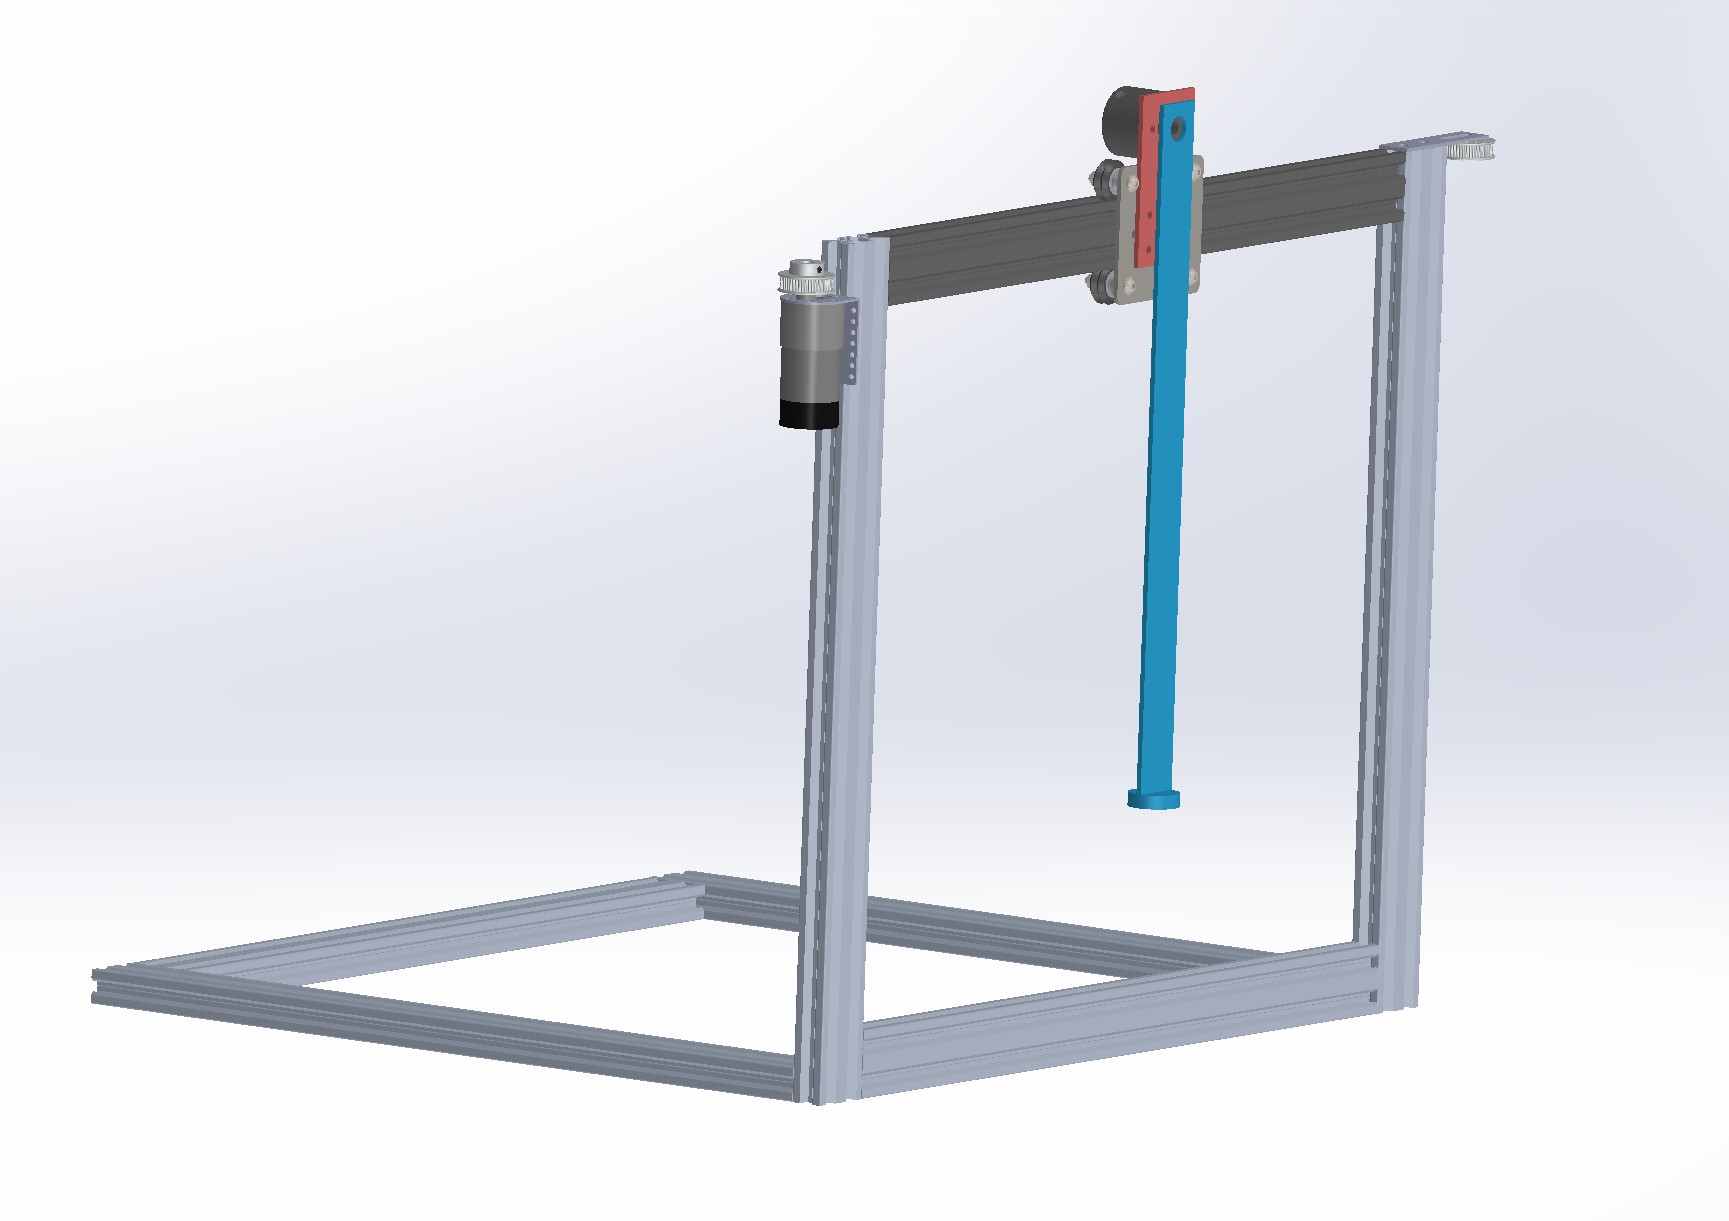
\includegraphics[scale=0.5]{praca_dyplomowa_wzor/figures/pendulum6.jpg}
    \caption{Poglądowy model 3D konstrukcji}
    \label{fig:konstrukcja}
\end{figure}

\subsection{Rama}
Do budowy konstrukcji urządzenia zostały wykorzystane aluminiowe profile typu V-Slot 2040, jak na rysunku \ref{fig:profil}. Przekrój profilu ma wymiary 20 x 40 mm, a jego boki mają charakterystyczne rowki w kształcie litery V. Rama została zbudowana z 3 profili o długości 500mm oraz 4 profili długości 250mm. Wszystkie elementy zostały ze sobą połączone dedykowanymi elementami wydrukowanymi na drukarce 3D oraz śrubami M4. Część elementów łączeniowych została znaleziona na stronie \textit{thingiverse.com}, na której udostępniane są modele 3D przygotowane z myślą o ich wydrukowaniu. Konstrukcja złożona w ten sposób charakteryzuje się dużą sztywnością, a przy tym niską masą.

\begin{figure}
    \centering
    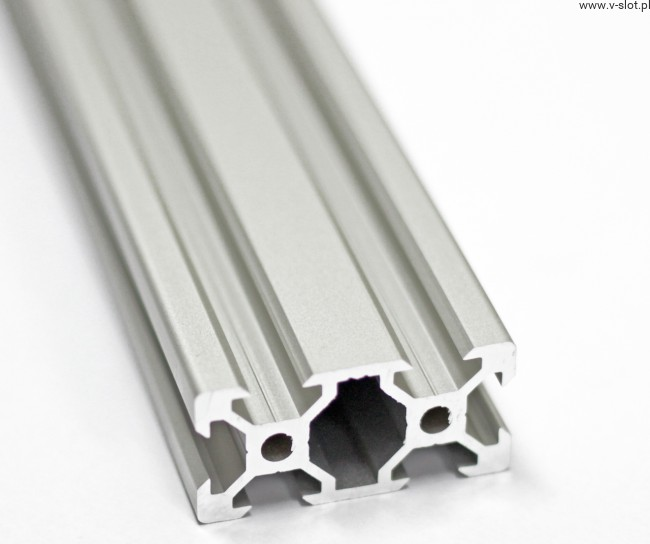
\includegraphics[scale=0.7]{praca_dyplomowa_wzor/figures/profil.jpg}
    \caption{Aluminiowy profil 2040}
    \texttt{Źródło: v-slot.pl}
    \label{fig:profil}
\end{figure}

\subsection{Układ jezdny}
Poruszający się wózek, popularnie nazywany karetką, został zbudowany na stalowej blasze, do którego przymocowano 4 łożyskowane rolki widoczne na rysunku \ref{fig:Rolka}, które są dedykowane do poruszania się po profilach V-Slot. Dodatkowo dolne rolki zostały zamontowane na tulejach mimośrodowych, dzięki czemu można regulować siłę docisku rolek do profilu. Do karetki przymocowany pas zębaty GT2 o szerokości 6mm, który z jednej strony porusza się po kole pasowym będącym napinaczem, a z drugiej po kole zębatym, które jest zamontowane na wale silnika. 

\begin{figure}
    \centering
    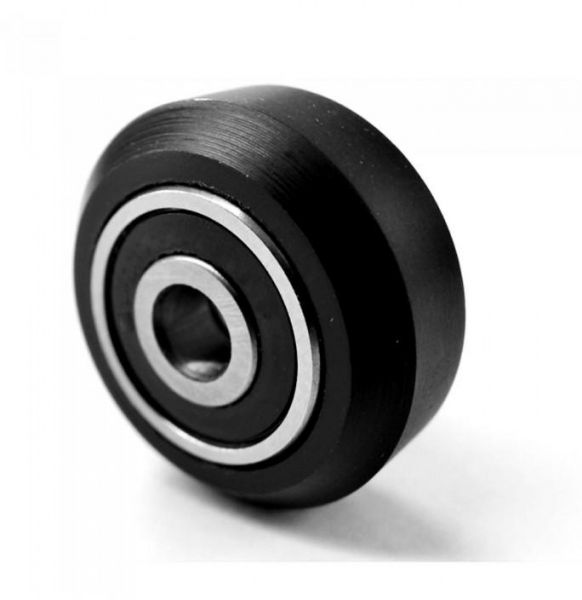
\includegraphics[scale=0.3]{praca_dyplomowa_wzor/figures/wheel.jpg}
    \caption{Rolka jezdna}
    \texttt{Źródło: black-frog.pl}
    \label{fig:Rolka}
\end{figure}

\section{Podzespoły}

\subsection{Mikrokontroler}
W urządzeniu został wykorzystany mikrokontroler firmy STMicroelectronics STM32F407 Discovery ukazany na rysunku \ref{fig:STM32}. Moduł wyposażony jest w 32-bitowy rdzeń ARM Cortex M4F. Maksymalne taktowanie mikroprocesora to 168 MHz, oferuje 1 MB pamięci flash oraz 192 kB pamięci RAM. Dodatkowo moduł jest wyposażony w dedykowany programator ST-LINK/V2, który pozwala również na debuggowanie. Mikrokontroler oferuje wiele programowalnych wejść i wyjść, a w tym między innymi w trybie wejścia sygnału enkodera czy wyjścia sygnału PWM. Moduł można zasilać zarówna z 5V jak i 3,3V. Płytka wraz ze sterownikiem silnika zostały przymocowane do konstrukcji przy pomocy samodzielnie zaprojektowanego uchwytu. 

\begin{figure}
    \centering
    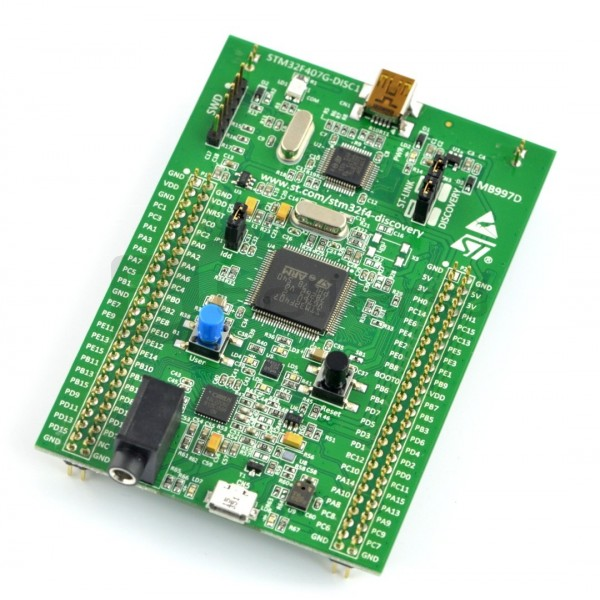
\includegraphics[scale=0.8]{praca_dyplomowa_wzor/figures/STM32F407.jpg}
    \caption{Mikrokontroler STM32F407 Discovery}
    \texttt{Źródło: botland.com.pl}
    \label{fig:STM32}
\end{figure}

\subsection{Enkoder}
Jako czujnik kąta odchylenia wahadła został wykorzystany enkoder DFRobot 400P/R, przedstawiony na rysunku \ref{fig:Enkoder}. Czujnik ma rozdzielczość 400 impulsów na każdy z 2 kanałów. Na wyjściach generowane są sygnały kwadraturowe, które są przesunięte w fazie względem siebie o 90\degree. W zależności od tego, na którym kanale najpierw pojawia się sygnał można rozróżnić, kierunek obrotów. Przy zliczaniu zliczaniu wszystkich zboczy sygnałów maksymalna rozdzielczość wynosi 1600 impulsów na obrót z czego wynika, ze jeden impuls to odchylenie o 0,225\degree. Enkoder może być zasilany napięciem od 4,8V do 24V. Sygnały wyjściowe czujnika są generowane przez tranzystory NPN w układzie otwartego kolektora, przez co linie sygnałowe wymagają podciągnięcia przez rezystory do dodatniej linii zasilania (pull-up).

\begin{figure}
    \centering
    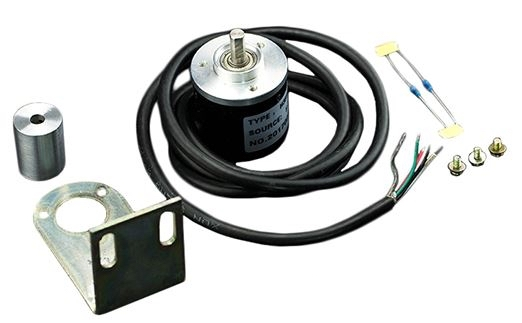
\includegraphics[scale=0.7]{praca_dyplomowa_wzor/figures/encoder.jpg}
    \caption{Enkoder DFRobot 400P/R}
    \texttt{Źródło: jsumo.com}
    \label{fig:Enkoder}
\end{figure}

\subsection{Silnik}
Do poruszania karetką został wykorzystany silnik prądu stałego Pololu 37Dx65L, ukazany nna rysunku \ref{fig:Silnik}. Napięcie zasilania silnika to 12V, minimalny pobór prądu to 0,2A, a maksymalny przy zatrzymaniu wału 5,5A. Silnik wyposażony jest w przekładnię o przełożeniu 6,25:1, dzięki której osiąga 1600 RPM przy nominalnym napięciu, a moment obrotowy wynosi 3kg/cm, czyli 0,294Nm. Dodatkowo silnik posiada własny enkoder o rozdzielczości 16 impulsów na obrót na każdym kanale co maksymalnie daje 64 impulsy na pełny obrót. Enkoder silnik może być zasilany napięciem od 3,5V do 20V. 

\begin{figure}
    \centering
    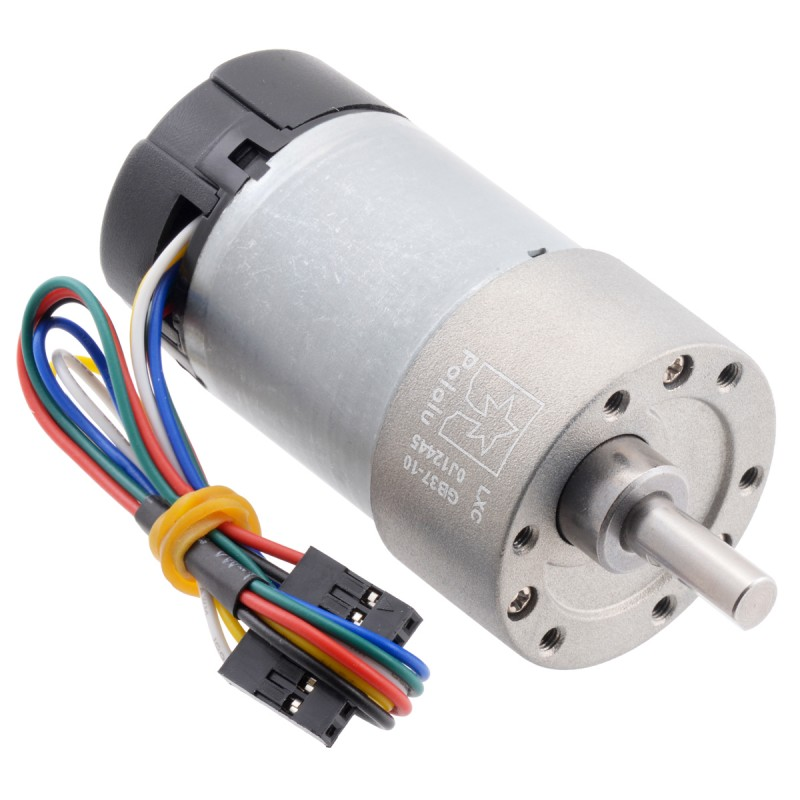
\includegraphics[scale=0.3]{praca_dyplomowa_wzor/figures/Pololu 37D.jpg}
    \caption{Silnik DC Pololu 37D}
    \texttt{Źródło: kamami.pl}
    \label{fig:Silnik}
\end{figure}

\subsection{Sterownik silnika}
Do sterowania silnikiem DC został wykorzystane moduł wyposażony w sterownik L298N, widoczny na rysunku \ref{fig:L298N}. Układ ten umożliwia sterowanie 2 silnikami dzięki dwóm osobnym kanałom. Napięcie zasilania silników może być dowolne z przedziału 4,8V do 46V, natomiast część logiczna wymaga zasilania napięciem 5V. Maksymalny prąd wyjściowy to 2A na każdy kanał, a dodatkowo kanały można połączyć ze sobą równolegle przez dwukrotnie zwiększy się wydajność prądowa. Moduł, dzięki zastosowaniu mostka H, pozwala sterować silnikiem w różnych kierunkach, a także stosować szybkie lub wolne hamowanie. Prędkość obrotów silnika można regulować sygnałem PWM.

\begin{figure}
    \centering
    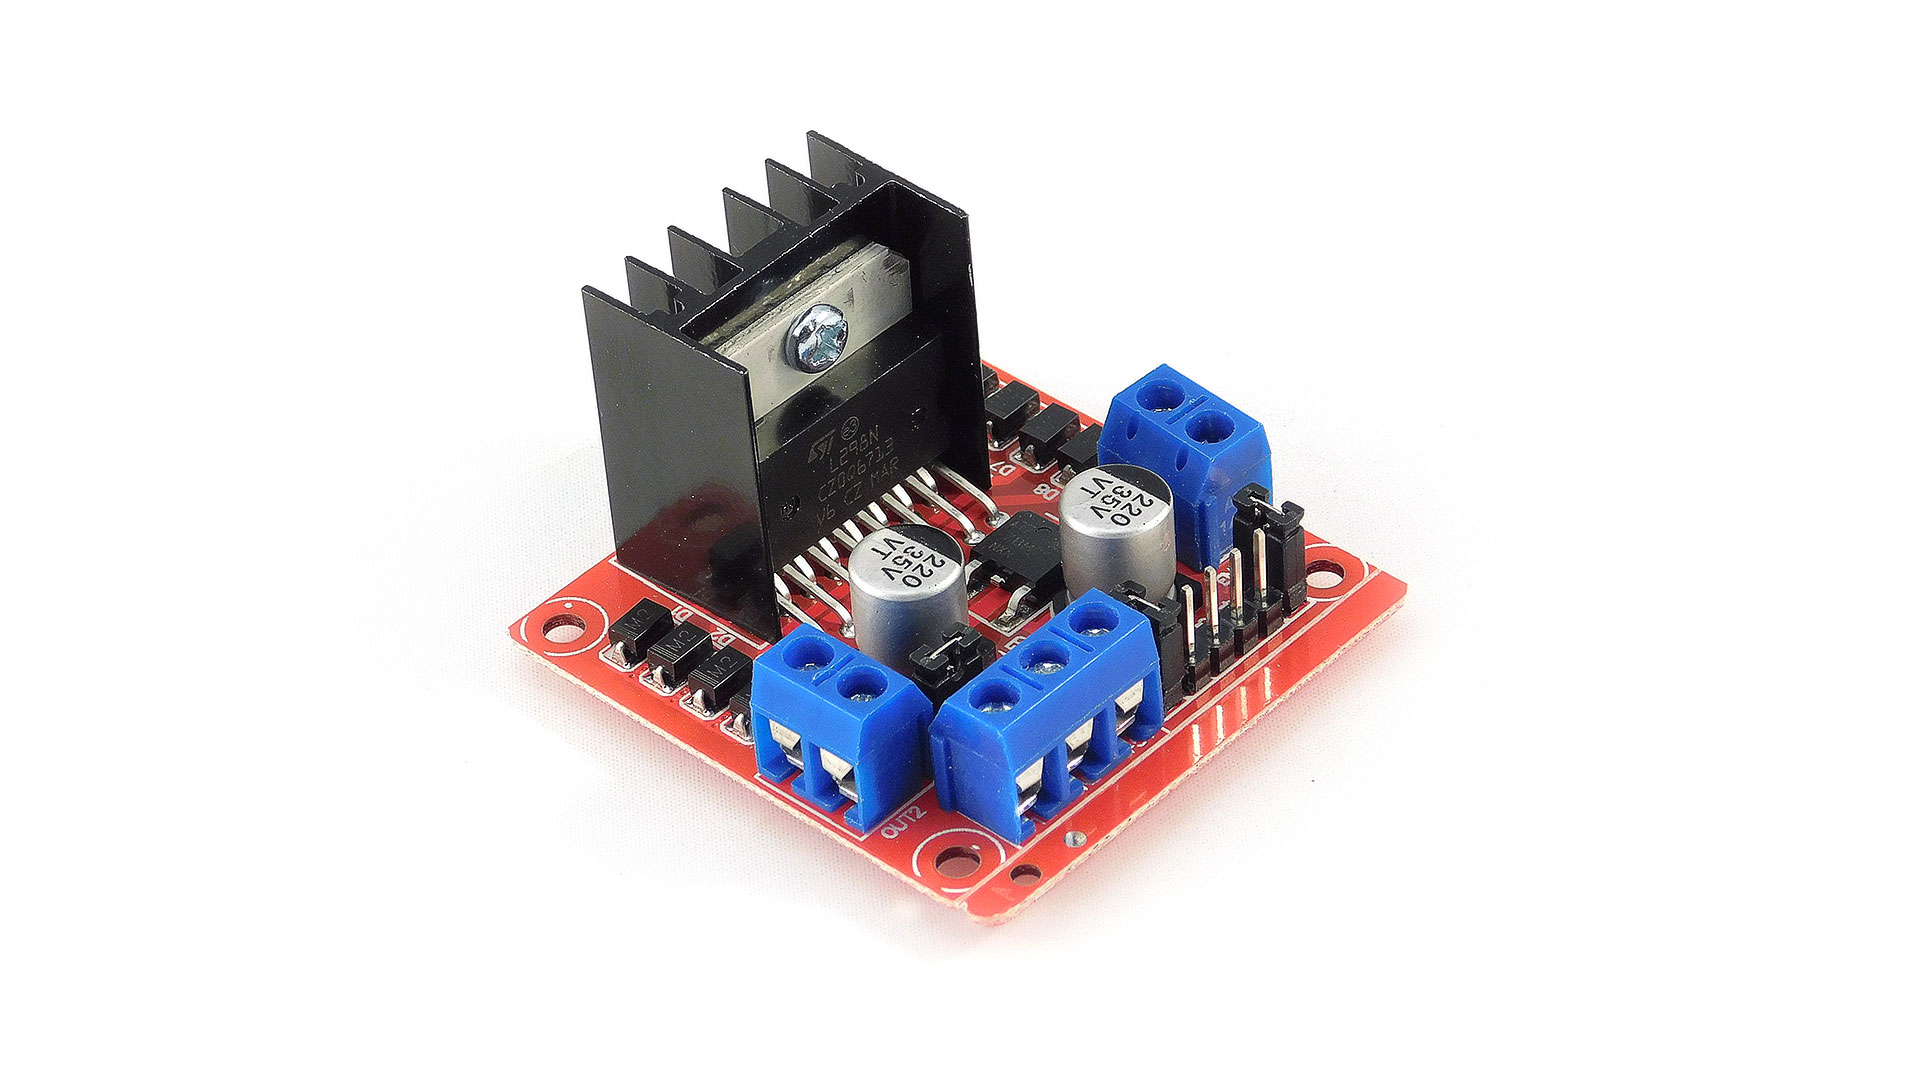
\includegraphics[scale=0.2]{praca_dyplomowa_wzor/figures/L298N.JPG}
    \caption{Sterownik silników DC L298N}
    \texttt{Źródło: botland.com.pl}
    \label{fig:L298N}
\end{figure}

\subsection{Zasilacz}
Do zasilania wszystkich podzespołów został użyty zasilacz komputerowy ATX o maksymalnej mocy 400W jak na rysunku \ref{fig:zasilacz}. Zaletą tego rozwiązania jest zapewnienie potrzebnych różnych napięć zasilania, bez potrzeby stosowania dodatkowych przetwornic. Zasilacz został umocowany do ramy przy pomocy samodzielnie zaprojektowanego i wydrukowanemu uchwytu.

\begin{figure}
    \centering
    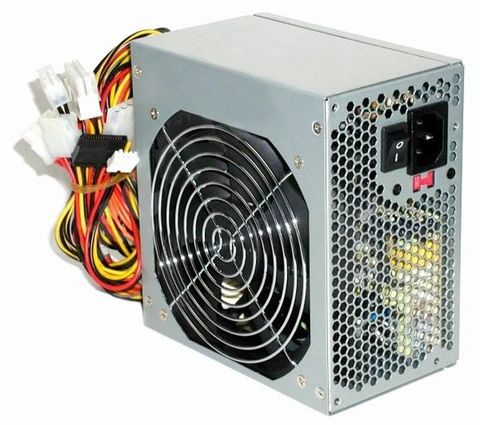
\includegraphics[scale=0.8]{praca_dyplomowa_wzor/figures/zasilacz.jpg}
    \caption{Zasilacz ATX 400W}
    \texttt{Źródło: internet-chorzow.pl}
    \label{fig:zasilacz}
\end{figure}




\chapter{Podsumowanie}

\cleardoublepage
\phantomsection
\addcontentsline{toc}{chapter}{\bibname}
\bibliographystyle{alphapl}
\bibliography{sources/bibliografia}
\markboth{\bibname}{\bibname}

%%spis rysunków
\cleardoublepage
\phantomsection
\addcontentsline{toc}{chapter}{\listfigurename}
\listoffigures
\markboth{\listfigurename}{\listfigurename}

\appendix
\chapter{Bąkiem malowane}

\end{document}
